% Fragment raportu - wykresy w folderze wykresy/ (eksport z wykresy.py)
\section{Skalowanie i analiza danych z giroskopów}

\subsection{Metodyka pomiarowa}
\akapit Kalibracja giroskopów polegała na wyznaczeniu napięcia spoczynkowego $U_{0}$ (gdy układ nie był w ruchu) oraz współczynnika skali $k$. Współczynnik ten wyznaczyliśmy metodą całkową, cztery razy wykonując obroty modułu o kąt $90^{\circ}$ wokół każdej z osi pomiarowych. Pozwoliło to na powiązanie pola pod wykresem napięcia z rzeczywistą zmianą kątową obiektu.

\subsection{Analiza prędkości kątowych i orientacji}
\akapit Podczas ruchu dowolnego zarejestrowaliśmy prędkości kątowe.

\akapit Głównym celem analizy było wyznaczenie orientacji obiektu (kątów Eulera: przechylenia $\Phi$, pochylenia $\Theta$ oraz odchylenia $\Psi$). W tym celu porównaliśmy dwa podejścia matematyczne. Pierwsze z nich oparte było na klasycznych równaniach kinematyki.

\begin{figure}[H]
    \centering
    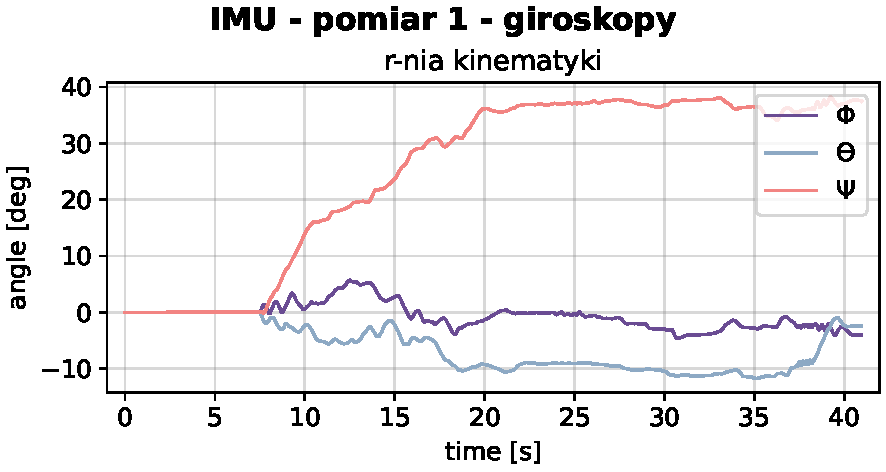
\includegraphics[width=0.85\textwidth]{wykresy/imu1_giroskopy_kinematyka.pdf}
    \caption{Orientacja obiektu wyznaczona poprzez całkowanie równań kinematyki.}
    \label{fig:kinematyka}
\end{figure}

\akapit Drugą metodą był rachunek kwaternionowy, który pozwala na uniknięcie osobliwości matematycznych i zapewnia większą stabilność numeryczną przy złożonych obrotach.

\begin{figure}[H]
    \centering
    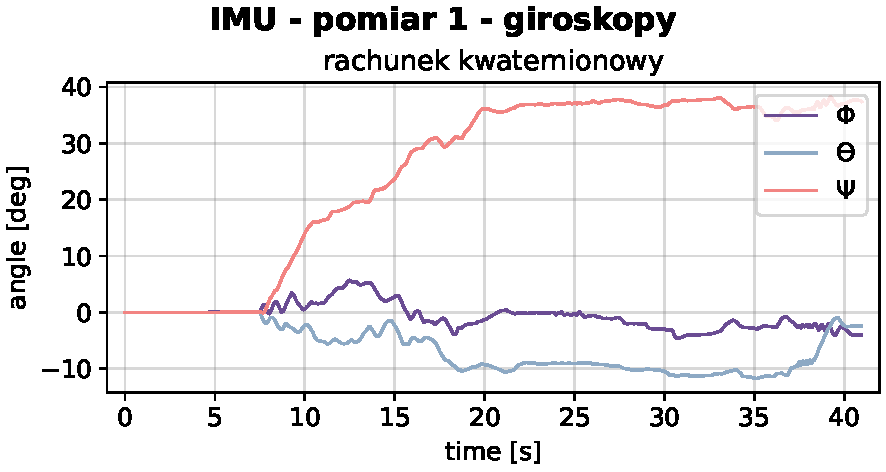
\includegraphics[width=0.85\textwidth]{wykresy/imu1_giroskopy_kwaterniony.pdf}
    \caption{Orientacja obiektu obliczona przy użyciu algorytmu kwaternionowego.}
    \label{fig:kwaterniony}
\end{figure}


\newpage
\section{Skalowanie i analiza danych z przyspieszeniomierzy}

\subsection{Opis wykonanych prac}
\akapit W pierwszej części ćwiczenia skupiliśmy się na wyznaczeniu parametrów kalibracyjnych dla trzech osi akcelerometru w module IMU-ZAIOL-01. Wykorzystaliśmy do tego celu wypoziomowaną płytę traserską. Proces polegał na statycznym ustawianiu modułu w taki sposób, aby każda z jego osi była skierowana kolejno zgodnie i przeciwnie do wektora grawitacji. Dzięki temu mogliśmy zarejestrować napięcia odpowiadające przyspieszeniu $\pm 1g$. Na tej podstawie wyznaczyliśmy współczynniki nachylenia oraz przesunięcia, co pozwoliło na przeliczenie sygnału z $V$ na $m/s^2$.

\subsection{Analiza wyników dla ruchu dowolnego}
\akapit Po przeprowadzeniu kalibracji zarejestrowaliśmy ruch swobodny urządzenia w przestrzeni.

\akapit Następnie, wykorzystując wyznaczone wcześniej stałe kalibracyjne, przeliczyliśmy te sygnały na fizyczne wartości przyspieszenia. Wynik tego procesu prezentuje kolejny wykres, na którym widać dynamiczne zmiany przyspieszeń wzdłuż osi X, Y oraz Z.

\begin{figure}[H]
    \centering
    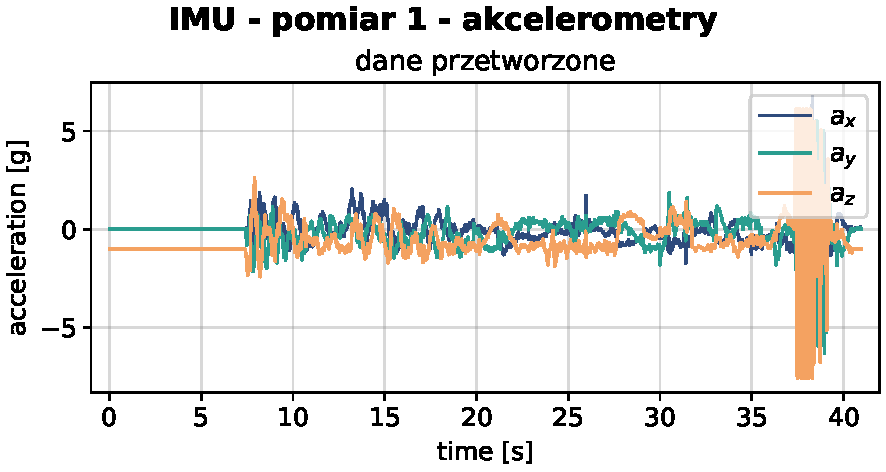
\includegraphics[width=0.85\textwidth]{wykresy/imu1_przyspieszenia.pdf}
    \caption{Przetworzone dane z akcelerometrów wyrażone w $m/s^2$.}
    \label{fig:acc_processed}
\end{figure}

\newpage
\section{Analiza danych z cyfrowego modułu IMU}

\subsection{Opis pomiarów}
\akapit W drugiej części ćwiczenia wykorzystaliśmy cyfrowy moduł IMU, który -- w odróżnieniu od układu analogowego -- zwraca dane już po wewnętrznym przeskalowaniu: przyspieszenia podawane są w jednostkach $g$, a prędkości kątowe w $^{\circ}/s$. Nie było zatem konieczności wyznaczania współczynników kalibracyjnych $k$ ani przesunięć napięciowych. Zarejestrowaliśmy trzy niezależne pomiary ruchu dowolnego z częstotliwością próbkowania $100\,\text{Hz}$. Każdy z nich rozpoczynał się od krótkiego postoju modułu, co pozwoliło wyznaczyć stałe przesunięcie zera giroskopów (jako średnią z pierwszej sekundy pomiaru) i odjąć je od zarejestrowanych prędkości kątowych.

\akapit Orientację modułu wyznaczyliśmy tymi samymi metodami co dla układu analogowego, tzn. całkując równania kinematyki oraz stosując rachunek kwaternionowy. W obu przypadkach przyjęliśmy zerowe warunki początkowe kątów Eulera.

\subsection{Pomiar 1}
\akapit Przebieg przyspieszeń oraz prędkości kątowych zarejestrowanych w pomiarze 1 przedstawiono na rysunkach \ref{fig:imu1_acc} i \ref{fig:imu1_gyro}.

\begin{figure}[H]
    \centering
    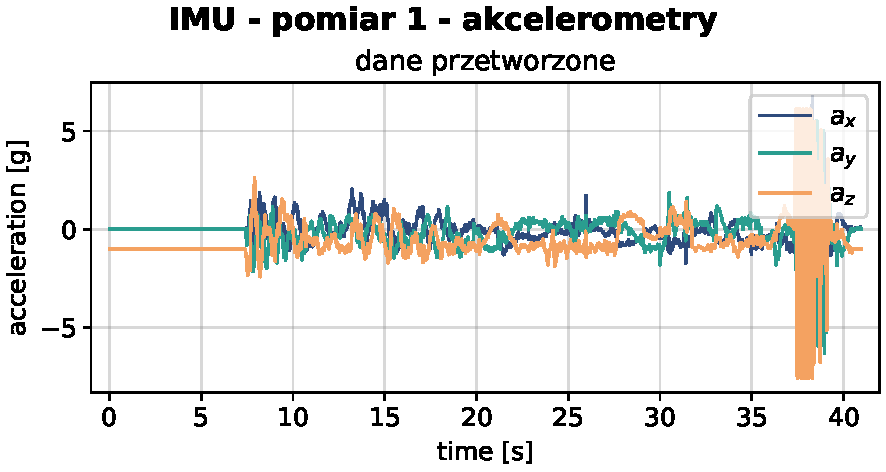
\includegraphics[width=0.85\textwidth]{wykresy/imu1_przyspieszenia.pdf}
    \caption{Przyspieszenia zarejestrowane przez moduł IMU -- pomiar 1.}
    \label{fig:imu1_acc}
\end{figure}
\hfill
\begin{figure}[H]
    \centering
    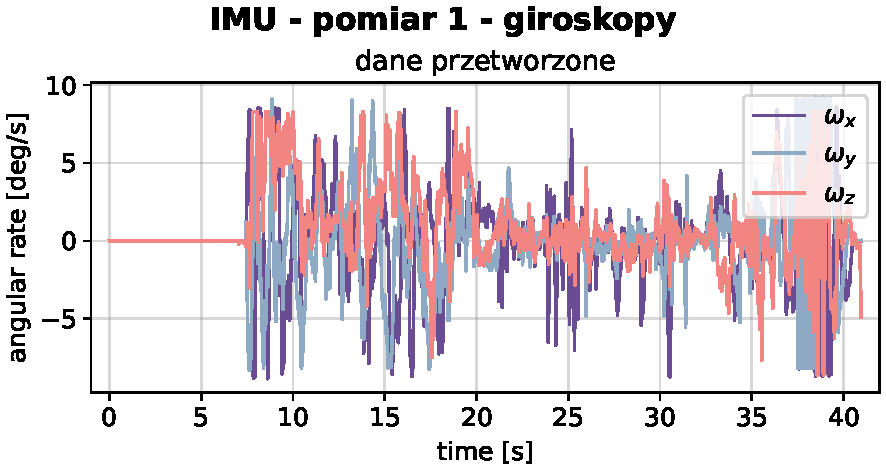
\includegraphics[width=0.85\textwidth]{wykresy/imu1_giroskopy.pdf}
    \caption{Prędkości kątowe zarejestrowane przez moduł IMU (po odjęciu przesunięcia zera) -- pomiar 1.}
    \label{fig:imu1_gyro}
\end{figure}

\akapit Orientację obiektu wyznaczoną z równań kinematyki i rachunkiem kwaternionowym pokazują odpowiednio rysunki \ref{fig:imu1_kin} i \ref{fig:imu1_kwat}.

\begin{figure}[H]
    \centering
    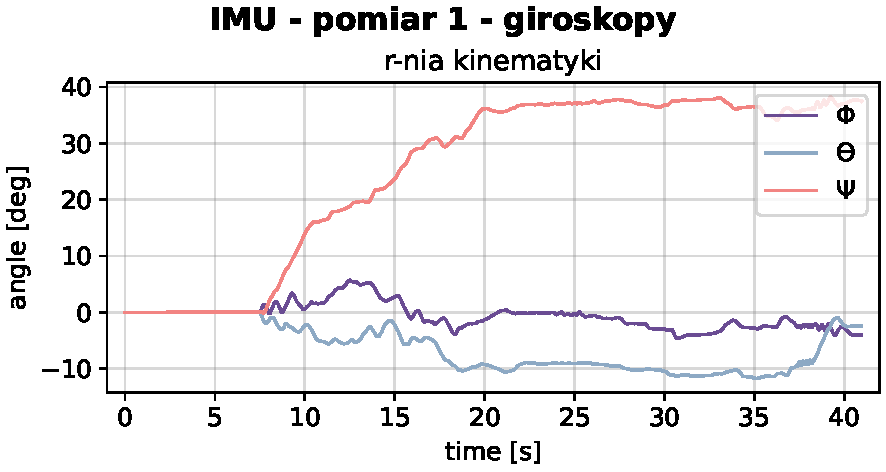
\includegraphics[width=0.85\textwidth]{wykresy/imu1_giroskopy_kinematyka.pdf}
    \caption{Orientacja modułu IMU wyznaczona z równań kinematyki -- pomiar 1.}
    \label{fig:imu1_kin}
\end{figure}
\hfill
\begin{figure}[H]
    \centering
    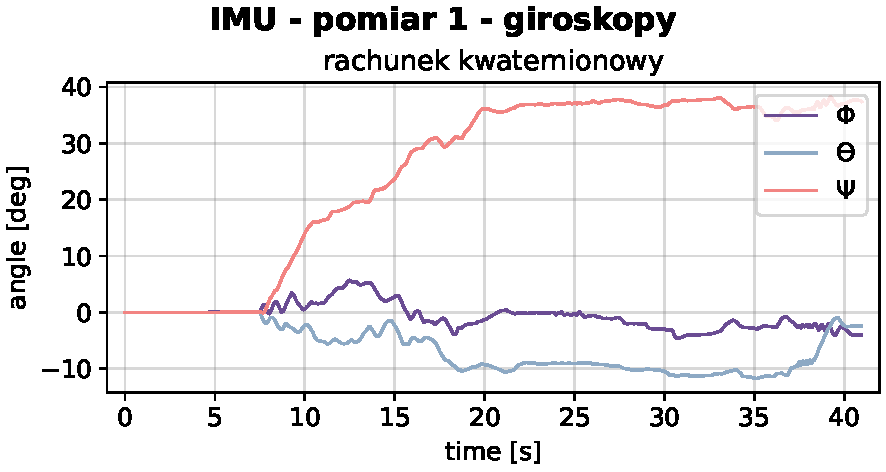
\includegraphics[width=0.85\textwidth]{wykresy/imu1_giroskopy_kwaterniony.pdf}
    \caption{Orientacja modułu IMU obliczona rachunkiem kwaternionowym -- pomiar 1.}
    \label{fig:imu1_kwat}
\end{figure}

\subsection{Pomiar 2}
\akapit Przebieg przyspieszeń oraz prędkości kątowych zarejestrowanych w pomiarze 2 przedstawiono na rysunkach \ref{fig:imu2_acc} i \ref{fig:imu2_gyro}.

\begin{figure}[H]
    \centering
    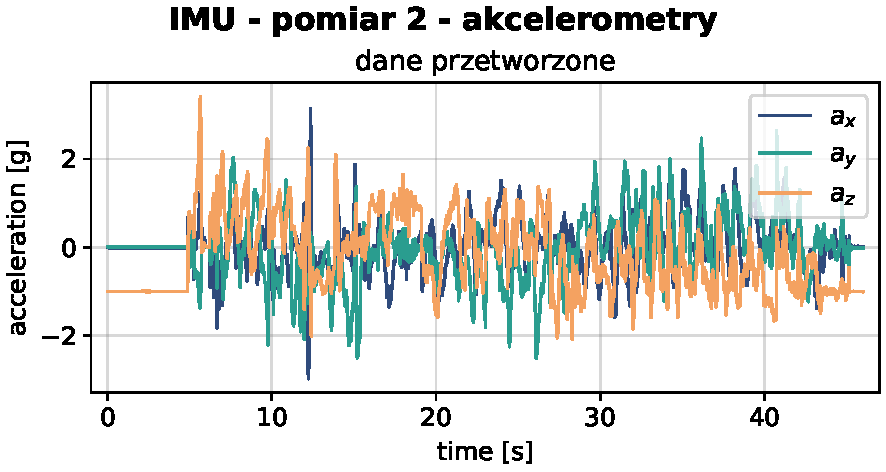
\includegraphics[width=0.85\textwidth]{wykresy/imu2_przyspieszenia.pdf}
    \caption{Przyspieszenia zarejestrowane przez moduł IMU -- pomiar 2.}
    \label{fig:imu2_acc}
\end{figure}
\hfill
\begin{figure}[H]
    \centering
    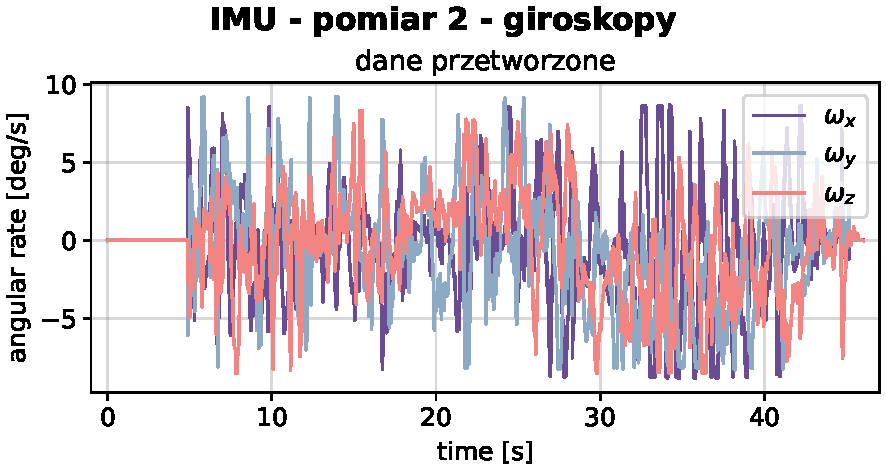
\includegraphics[width=0.85\textwidth]{wykresy/imu2_giroskopy.pdf}
    \caption{Prędkości kątowe zarejestrowane przez moduł IMU (po odjęciu przesunięcia zera) -- pomiar 2.}
    \label{fig:imu2_gyro}
\end{figure}

\akapit Orientację obiektu wyznaczoną z równań kinematyki i rachunkiem kwaternionowym pokazują odpowiednio rysunki \ref{fig:imu2_kin} i \ref{fig:imu2_kwat}.

\begin{figure}[H]
    \centering
    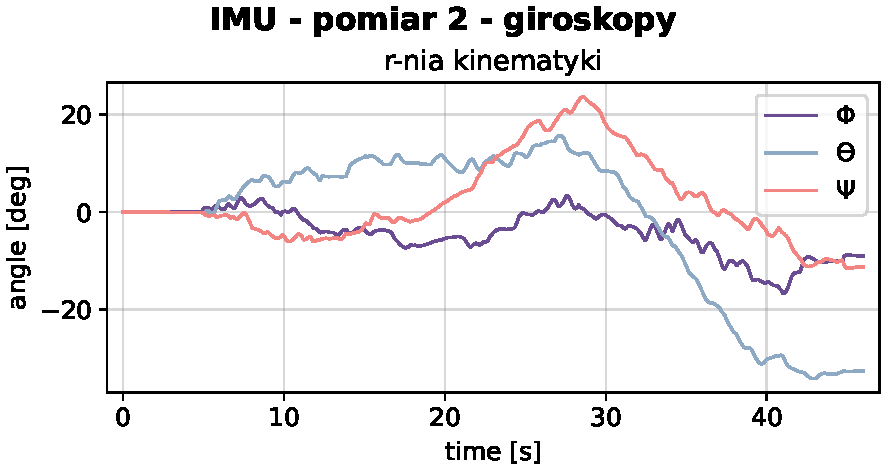
\includegraphics[width=0.85\textwidth]{wykresy/imu2_giroskopy_kinematyka.pdf}
    \caption{Orientacja modułu IMU wyznaczona z równań kinematyki -- pomiar 2.}
    \label{fig:imu2_kin}
\end{figure}
\hfill
\begin{figure}[H]
    \centering
    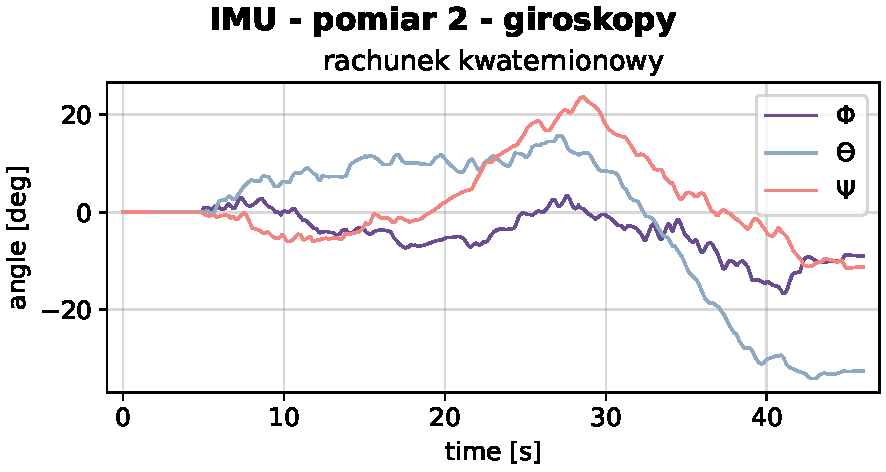
\includegraphics[width=0.85\textwidth]{wykresy/imu2_giroskopy_kwaterniony.pdf}
    \caption{Orientacja modułu IMU obliczona rachunkiem kwaternionowym -- pomiar 2.}
    \label{fig:imu2_kwat}
\end{figure}

\subsection{Pomiar 3}
\akapit Przebieg przyspieszeń oraz prędkości kątowych zarejestrowanych w pomiarze 3 przedstawiono na rysunkach \ref{fig:imu3_acc} i \ref{fig:imu3_gyro}.

\begin{figure}[H]
    \centering
    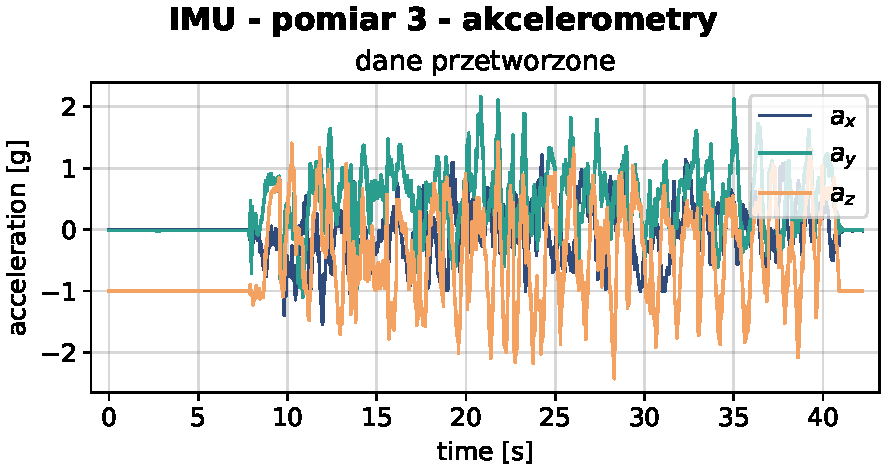
\includegraphics[width=0.85\textwidth]{wykresy/imu3_przyspieszenia.pdf}
    \caption{Przyspieszenia zarejestrowane przez moduł IMU -- pomiar 3.}
    \label{fig:imu3_acc}
\end{figure}
\hfill
\begin{figure}[H]
    \centering
    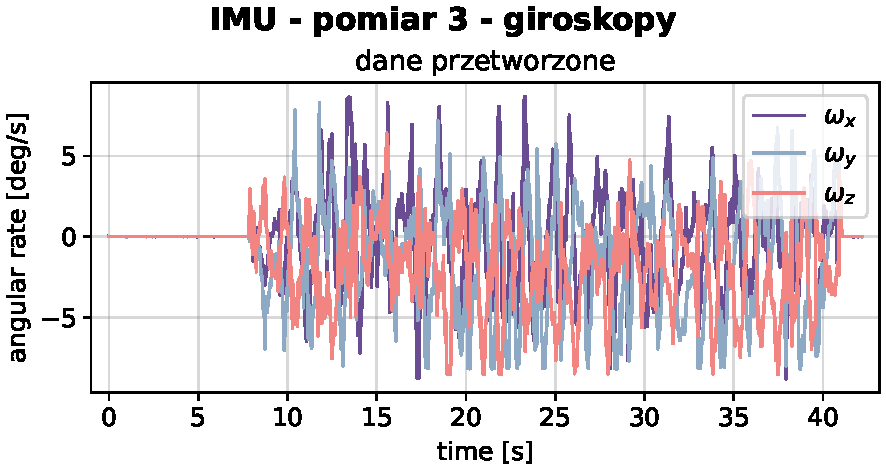
\includegraphics[width=0.85\textwidth]{wykresy/imu3_giroskopy.pdf}
    \caption{Prędkości kątowe zarejestrowane przez moduł IMU (po odjęciu przesunięcia zera) -- pomiar 3.}
    \label{fig:imu3_gyro}
\end{figure}

\akapit Orientację obiektu wyznaczoną z równań kinematyki i rachunkiem kwaternionowym pokazują odpowiednio rysunki \ref{fig:imu3_kin} i \ref{fig:imu3_kwat}.

\begin{figure}[H]
    \centering
    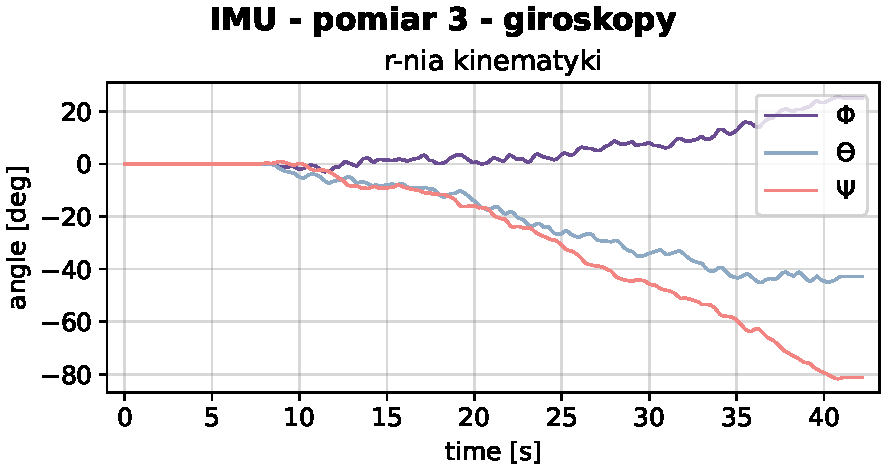
\includegraphics[width=0.85\textwidth]{wykresy/imu3_giroskopy_kinematyka.pdf}
    \caption{Orientacja modułu IMU wyznaczona z równań kinematyki -- pomiar 3.}
    \label{fig:imu3_kin}
\end{figure}
\hfill
\begin{figure}[H]
    \centering
    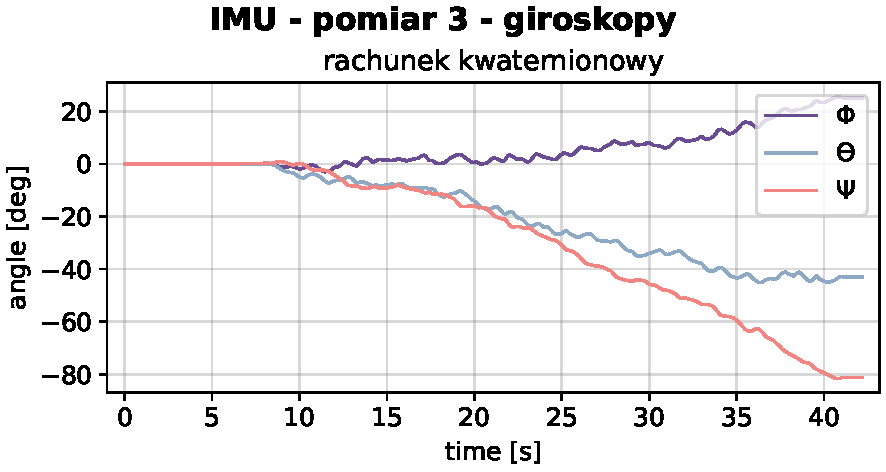
\includegraphics[width=0.85\textwidth]{wykresy/imu3_giroskopy_kwaterniony.pdf}
    \caption{Orientacja modułu IMU obliczona rachunkiem kwaternionowym -- pomiar 3.}
    \label{fig:imu3_kwat}
\end{figure}
